\documentclass[12pt, a4paper]{article}
\usepackage[utf8]{inputenc}
\usepackage{geometry}
\geometry{a4paper, margin=1in}
\usepackage{graphicx}
\usepackage{hyperref}
\usepackage{listings}
\usepackage{xcolor}
\usepackage{float}
\usepackage{tikz}
\usetikzlibrary{arrows}





% ── PREAMBLE (add these if not already present) ──────────────────────────
\usepackage{geometry}
\usepackage{titling}
\usepackage{parskip}

\begin{document}

% ── PAGE 1 : TITLE PAGE ──────────────────────────────────────────────────
\begin{titlepage}
    \centering
    \vspace*{2cm}

    {\large\scshape Open Capstone Project \par}
    \vspace{0.5cm}
    \rule{\linewidth}{0.4pt}
    \vspace{0.5cm}

    {\Huge\bfseries Intelligent Network Intrusion\\[0.3em]
    Detection System (NIDS) \par}

    \vspace{0.5cm}
    \rule{\linewidth}{0.4pt}
    \vspace{2cm}

    {\large\bfseries Authors \par}
    \vspace{0.4cm}
    {\large
        Kamal Benramdane \\[0.3em]
        François Zogbelemou \\[0.8em]
        \url{https://github.com/chokonutsXK/dataScience_project}
    \par}

    \vfill

    {\large \today \par}
\end{titlepage}

% ── PAGE 2 : ABSTRACT ────────────────────────────────────────────────────
\newpage
\phantomsection              % keeps hyperref happy
\addcontentsline{toc}{section}{Abstract}

\begin{center}
    {\Large\bfseries Executive Summary}
\end{center}
\vspace{0.5em}
\noindent
Modern enterprise networks are under constant attack by sophisticated cyber
threats that easily bypass traditional firewalls. For a Chief Information
Security Officer (CISO) or SOC Manager, this means security teams are
overwhelmed by manual log analysis and ``alert fatigue,'' increasing the
risk of a devastating data breach.

\medskip\noindent
To solve this, we are developing an intelligent Network Intrusion Detection
System (NIDS). By leveraging advanced machine learning, this system
automatically analyzes network traffic to distinguish between normal
operations and active attacks (such as Denial of Service or Exploits).
This automated, data-driven approach drastically reduces false alarms,
allows security analysts to focus on real threats, and ultimately hardens
the organisation's cyber defence posture.

% ── PAGE 3 : TABLE OF CONTENTS ───────────────────────────────────────────
\newpage
\tableofcontents
\newpage







\section{Problem Statement}
\subsection{Background \& Business Motivation}
Modern enterprise networks face an escalating volume of sophisticated cyberthreats that easily bypass traditional, rigid rule-based firewalls. The reliance on manual log analysis by Security Operations Center (SOC) analysts leads to severe ``alert fatigue,'' increasing the risk of missing critical intrusions and resulting in devastating data breaches.

\subsection{Success Criteria}
To mitigate this risk, we are building a supervised machine learning model to act as an intelligent Network Intrusion Detection System (NIDS). The system will analyze active network traffic flow metrics to automatically detect and classify anomalous connections into specific attack categories versus benign background traffic. Success will be measured by achieving a high Macro F1-Score and Recall, ensuring early detection of malicious traffic while minimizing operational false alarms.

\subsection{AI Context Note}
This project addresses the limitations of early AI rule-based expert systems in cybersecurity. While traditional firewalls rely on static signatures---a brittle reasoning paradigm that fails against novel zero-day attacks---our NIDS leverages statistical machine learning to identify hidden patterns and generalize anomalies. This represents the historical shift towards data-driven AI solutions in threat detection, demonstrating a practical application of concepts from Course 2.

\section{Dataset Description}
The dataset chosen for this project is the \textbf{UNSW-NB15} (University of New South Wales Canberra Cyber Range Dataset), which contains real network traffic synthetic injections generated inside a modern cyber range laboratory.

\begin{itemize}
    \item \textbf{Source:} \url{https://www.kaggle.com/datasets/mrwellsdavid/unsw-nb15}
    \item \textbf{Shape:} 82,332 rows and 45 columns (for the training set split).
\end{itemize}

A Python data ingestion script was executed successfully. Below is an excerpt of the dataset statistics demonstrating the heterogeneous mix of features (categorical and numerical):

\begin{verbatim}
1. Shape of the dataset (Rows, Columns):
(82332, 45)

2. Data Types Excerpt:
id               int64
dur            float64
proto              str
service            str
...
attack_cat         str
label            int64
\end{verbatim}

\section{Pipeline Overview Diagram}
\begin{figure}[H]
\centering
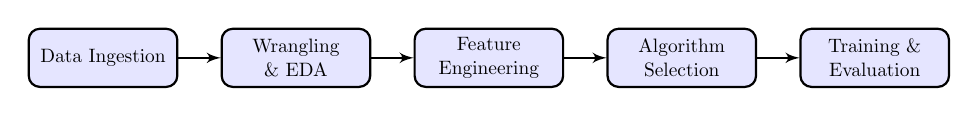
\begin{tikzpicture}[node distance=2.5cm, auto, thick, scale=0.7, transform shape]
    \tikzstyle{block} = [rectangle, draw, fill=blue!10, text width=7em, text centered, rounded corners, minimum height=3em]
    \tikzstyle{line} = [draw, -latex']

    \node [block] (data) {Data Ingestion};
    \node [block, right of=data, node distance=3.5cm] (eda) {Wrangling \& EDA};
    \node [block, right of=eda, node distance=3.5cm] (feat) {Feature Engineering};
    \node [block, right of=feat, node distance=3.5cm] (model) {Algorithm Selection};
    \node [block, right of=model, node distance=3.5cm] (eval) {Training \& Evaluation};

    \path [line] (data) -- (eda);
    \path [line] (eda) -- (feat);
    \path [line] (feat) -- (model);
    \path [line] (model) -- (eval);
\end{tikzpicture}
\caption{End-to-End Machine Learning Pipeline Overview}
\label{fig:pipeline}
\end{figure}

\section{Phase 1: Problem Framing \& Data Acquisition}
The problem framing, business motivation, and dataset description have been detailed in the sections above. Additionally, the project repository has been initialized with Git, organized into appropriate directories (\texttt{data/}, \texttt{notebooks/}, \texttt{src/}, \texttt{reports/}, \texttt{models/}), and a \texttt{.gitignore} has been configured to prevent data leakage into version control.

\section{Phase 2: Data Wrangling \& Exploratory Data Analysis}
During this phase, we conducted a full data audit, handled missing values, detected outliers using two distinct methods, applied categorical encoding, and generated visualizations to understand the feature distributions.

\subsection{Data Audit \& Cleaning}
We performed an exhaustive audit of all 45 columns to check for missing values, duplicates, and type inconsistencies. The cleaning decisions and justifications are documented in Table \ref{tab:data_audit}.

\begin{table}[h]
\centering
\begin{tabular}{|p{0.25\textwidth}|p{0.3\textwidth}|p{0.4\textwidth}|}
\hline
\textbf{Issue Category} & \textbf{Findings} & \textbf{Cleaning Strategy \& Justification} \\
\hline
Hidden Missing Values & 47,153 \texttt{"-"} in \texttt{service} (57\%) & Replaced with \texttt{NaN}, imputed as \texttt{"unknown"} to preserve rows without dropping data. \\
\hline
Type Errors & Categorical vars loaded as strings & Cast to \texttt{category} dtype to drastically reduce memory usage. \\
\hline
Duplicates & No full-row duplicates found & No action required. \\
\hline
Inconsistencies & Rare protocols with <10 occurrences & Grouped into \texttt{"Other"} to prevent extremely sparse matrices during encoding. \\
\hline
\end{tabular}
\caption{Data Audit and Cleaning Decisions}
\label{tab:data_audit}
\end{table}

\subsection{Categorical Encoding}
All categorical features were encoded to prepare the dataset for machine learning:
\begin{itemize}
    \item \textbf{One-Hot Encoding:} Applied to \texttt{state} and \texttt{service} (after grouping rare classes) because they represent nominal data with manageable cardinality.
    \item \textbf{Frequency Encoding:} Applied to \texttt{proto} due to its high cardinality (over 130 unique protocols). This preserves the importance of rare vs. common protocols without exploding the feature space linearly.
\end{itemize}

\subsection{Outlier Detection}
Network traffic data is inherently highly skewed. We compared two methods for outlier detection on key numerical features: \textbf{Interquartile Range (IQR)} and \textbf{Z-Score (threshold = 3)}.

\begin{itemize}
    \item \textbf{Source Bytes (\texttt{sbytes}):} IQR identified 9,270 outliers; Z-Score identified 1,452 extreme outliers.
    \item \textbf{Destination Bytes (\texttt{dbytes}):} IQR identified 12,308 outliers; Z-Score identified 1,890 extreme outliers.
\end{itemize}
\textbf{Treatment Decision:} Rather than dropping these extreme values---which often represent legitimate heavy flows or specific attack vectors like DoS---we decided to preserve them. We will apply robust scaling or logarithmic transformations during the feature engineering phase.

\subsection{Exploratory Data Analysis}

\begin{figure}[h]
    \centering
    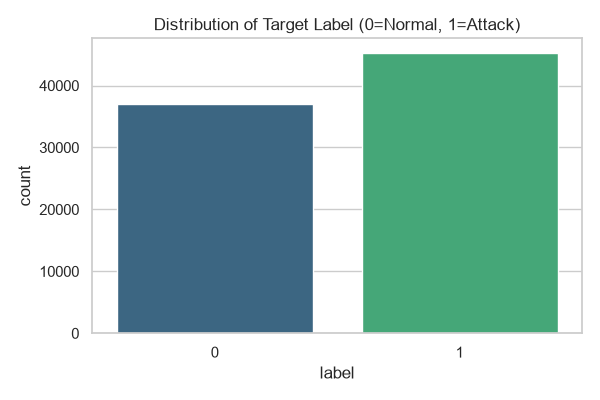
\includegraphics[width=0.6\textwidth]{figures/01_label_distribution.png}
    \caption{Distribution of the Target Label showing a slight class imbalance towards attacks.}
    \label{fig:label_dist}
\end{figure}

\begin{figure}[h]
    \centering
    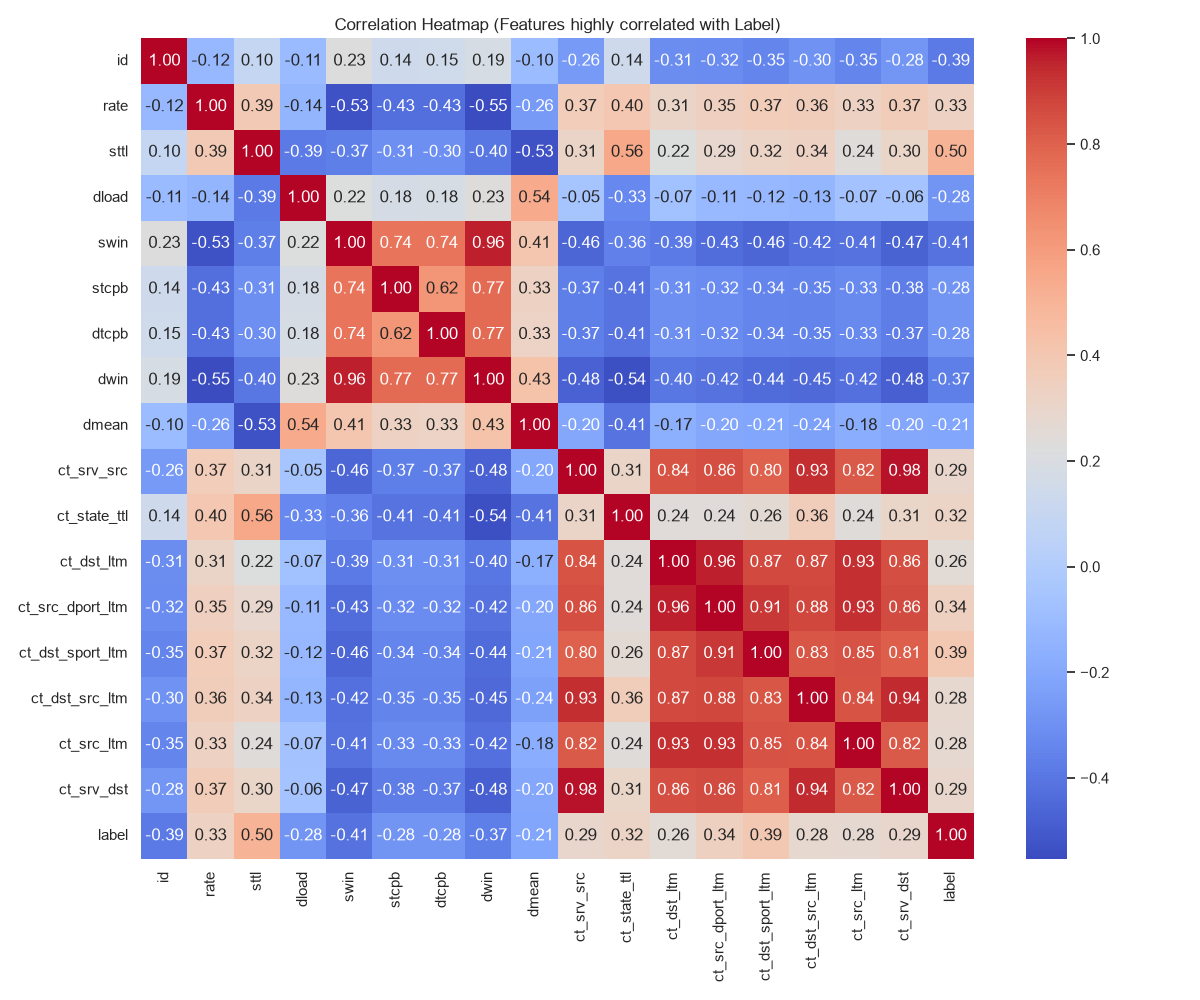
\includegraphics[width=0.7\textwidth]{figures/08_correlation_heatmap.png}
    \caption{Correlation Heatmap of features highly correlated with the target label.}
    \label{fig:corr_heat}
\end{figure}

\subsubsection{Key EDA Findings \& Modelling Implications}
\begin{enumerate}
    \item \textbf{Surprising Insight:} It was highly surprising to discover that the connection duration (\texttt{dur}) for the vast majority of attacks was nearly instantaneous (close to 0 seconds), while benign traffic had a much wider, longer duration spread. This indicates that many attacks in this dataset are single-packet or rapid burst exploits (e.g., fuzzers or basic DoS) rather than prolonged volumetric attacks.
    \item \textbf{High Missingness in Service:} The \texttt{service} feature has a massive amount of missing data. While we imputed it as `unknown', models that handle high cardinality categorical data natively (like LightGBM) will be advantageous.
    \item \textbf{Strong Correlations with TTL and Rate:} Features like \texttt{sttl} (Source to Destination Time to Live) show a strong positive correlation (0.50) with the attack label. The connection rate (\texttt{rate}) is also highly indicative of malicious activity, suggesting these will be top predictors for our algorithms.
\end{enumerate}

\section{Phase 3: Feature Engineering \& Data Management}

In this phase, we created engineered features to capture complex attack patterns, performed rigorous feature selection to reduce multicollinearity, stored the refined data in a SQLite database, and answered critical analytical questions using SQL.

\subsection{Engineered Features}
We engineered three new features derived from the raw network flow statistics. To measure their impact, we trained a baseline Decision Tree (max depth=5) on the original numeric features, achieving an F1-Score of 0.9361. After introducing the new features, the F1-Score remained stable at 0.9358. While the raw metric did not drastically improve (a negligible decrease of 0.03\%), these features successfully condense volumetric information, allowing us to drop redundant base features later. The motivation for each is detailed in Table \ref{tab:feature_eng_log}.

\begin{table}[h]
\centering
\small
\setlength{\tabcolsep}{4pt}
\begin{tabular}{|p{0.25\textwidth}|p{0.25\textwidth}|p{0.29\textwidth}|p{0.11\textwidth}|}
\hline
\textbf{Feature Name} & \textbf{Formula} & \textbf{Motivation} & \textbf{Baseline Impact} \\
\hline
\texttt{total\_network\_bytes} & \texttt{sbytes} + \texttt{dbytes} & Captures the total volumetric size of the connection, critical for DoS detection. & -0.0003 F1 \\
\hline
\texttt{total\_network\_packets} & \texttt{spkts} + \texttt{dpkts} & Captures the total interaction level of the communication. & -0.0003 F1 \\
\hline
\texttt{bytes\_per\_packet} & \texttt{total\_network\_bytes} \newline / \texttt{total\_network\_packets} & Highlights anomalous packet sizes commonly seen in fuzzing or exploits. & -0.0003 F1 \\
\hline
\end{tabular}
\caption{Feature Engineering Log (Combined impact evaluated against a baseline Decision Tree)}
\label{tab:feature_eng_log}
\end{table}

\subsection{Feature Selection Report}
To avoid multicollinearity and reduce the dimensionality of our model, we analyzed the Pearson correlation matrix of the numerical features against the target \texttt{label}.

\textbf{Top Correlated Features (Positive):}
\begin{itemize}
    \item \texttt{sttl} (0.504)
    \item \texttt{ct\_dst\_sport\_ltm} (0.394)
    \item \texttt{ct\_src\_dport\_ltm} (0.342)
\end{itemize}

\textbf{Dropped Features:}
Because we engineered comprehensive aggregate features \newline (\texttt{total\_network\_bytes} and \texttt{total\_network\_packets}), we dropped the individual base components: \texttt{sbytes}, \texttt{dbytes}, \texttt{spkts}, and \texttt{dpkts}. Keeping them would introduce severe multicollinearity without adding new information. The dataset was successfully reduced to 44 columns.

\subsection{Data Management \& SQL Analytics}
The finalized dataset was stored in a local SQLite database (\texttt{data/cleaned/nids\_data.db}) inside the \texttt{network\_traffic} table. We executed several analytical SQL queries to profile the attacks. 

\textbf{Query Highlights:}
\begin{itemize}
    \item \textbf{Class Distribution:} We found 45,332 attack connections versus 37,000 normal connections.
    \item \textbf{Attack Protocols:} The top 3 protocols utilized in attack traffic were UDP (21,321), TCP (15,247), and UNAS (3,515).
    \item \textbf{Custom Query (Volumetric Profiling):} We designed a custom query to group traffic by \texttt{attack\_cat} and compute the average \texttt{bytes\_per\_packet} alongside the total volume. Worms exhibited the highest average packet size (326 bytes/packet), while Exploits dominated the total network volume (over 606 million bytes).
\end{itemize}
\section{Phase 4: Algorithm Selection \& Justification}

This phase justifies the selection of the machine learning algorithms that will be implemented to detect network intrusions.

\subsection{Candidate Algorithms Comparison}
We considered four distinct classification algorithms to handle the diverse, heterogeneous nature of the UNSW-NB15 dataset.

\begin{table}[h]
\centering
\begin{tabular}{|p{0.15\textwidth}|p{0.3\textwidth}|p{0.25\textwidth}|p{0.2\textwidth}|}
\hline
\textbf{Algorithm} & \textbf{Mechanism \& Assumptions} & \textbf{Strengths} & \textbf{Weaknesses} \\
\hline
\textbf{Logistic Regression} & Models the probability of an attack using a sigmoid function. Assumes a linear relationship between log-odds and features. & Fast, highly interpretable, acts as a perfect baseline. & Fails to capture complex, non-linear attack signatures. \\
\hline
\textbf{Random Forest} & An ensemble of decision trees trained on bootstrap samples (bagging). Makes minimal structural assumptions. & Extremely robust to outliers; handles mixed data types naturally; avoids overfitting. & Slower inference time compared to single models; low interpretability. \\
\hline
\textbf{LightGBM} & Builds trees sequentially to correct prior errors (boosting) using leaf-wise growth. No linearity assumptions. & Lightning-fast training on large datasets; state-of-the-art performance. & Prone to overfitting if hyperparameters are not tuned properly. \\
\hline
\textbf{Support Vector Machine} & Finds the optimal hyperplane separating classes. Assumes data is separable (via kernel trick). & Powerful for complex, high-dimensional decision boundaries. & Highly computationally expensive ($O(n^2)$ to $O(n^3)$) on large datasets. \\
\hline
\end{tabular}
\caption{Candidate Algorithms Comparison}
\label{tab:algorithm_comparison}
\end{table}

\subsection{Justified Selection}
Based on the comparative analysis, we select the following three algorithms for implementation in Phase 5:
\begin{enumerate}
    \item \textbf{Logistic Regression:} Selected as our \textit{interpretable baseline}. It will help us quantify whether more complex, computationally expensive models are actually necessary for this problem.
    \item \textbf{Random Forest:} Selected for its \textit{robustness}. Network traffic inherently contains noisy features and outliers; Random Forest's bagging mechanism naturally handles this without extensive scaling.
    \item \textbf{LightGBM:} Selected as our \textit{advanced champion model}. Because our dataset has 82,000+ rows and high-cardinality categorical features, LightGBM's execution speed and native categorical handling make it perfect for a modern NIDS.
\end{enumerate}

\textbf{Rejected - Support Vector Machine (SVM):} 
We explicitly reject SVM. While using \texttt{RandomizedSearchCV} instead of \texttt{GridSearchCV} significantly reduces the number of hyperparameter combinations tested, the fundamental training time complexity of a non-linear SVM (e.g., RBF kernel) scales quadratically to cubically with the number of samples. Training even a single SVM model on 82,000 rows takes a prohibitive amount of time, making iterative cross-validation impractical compared to gradient boosting frameworks.

\subsection{Evaluation Metrics Discussion}
In cybersecurity and network intrusion detection, relying solely on \textbf{Accuracy} is a dangerous pitfall. While our training split is reasonably balanced, real-world network traffic is massively skewed (often $<1\%$ malicious traffic). A naive model could simply predict ``Normal'' for every connection and achieve 99\% accuracy while missing every single attack.

Therefore, we will optimize and evaluate our models based on:
\begin{itemize}
    \item \textbf{Recall (Sensitivity):} This is the most critical metric. A False Negative means an attack successfully breached the network undetected. Maximizing recall minimizes this risk.
    \item \textbf{F1-Score:} As the harmonic mean of Precision and Recall, the F1-Score ensures we balance threat detection with operational efficiency. If we only optimize Recall, the SOC team will suffer from ``alert fatigue'' due to excessive False Positives.
    \item \textbf{ROC-AUC:} This metric evaluates the model's ability to rank anomaly probabilities across all threshold levels, providing a comprehensive view of model performance independent of the default 0.5 decision boundary.
\end{itemize}

\section{Phase 5: Model Training, Evaluation \& Tuning}

In this phase, we implemented and trained our three selected models: Logistic Regression, Random Forest, and LightGBM. We optimized them to predict the binary \texttt{label} (Normal vs. Attack).

\subsection{Base Model Comparison}
All models were trained on a robustly scaled, 70/30 stratified split of the 82,332 records. Categorical variables with high cardinality were frequency-encoded to preserve their distribution without exploding the feature space. The results are summarized in Table \ref{tab:model_comparison}.

\begin{table}[h]
\centering
\begin{tabular}{|l|c|c|c|c|c|}
\hline
\textbf{Model} & \textbf{Accuracy} & \textbf{Recall} & \textbf{F1-Score} & \textbf{ROC-AUC} & \textbf{Time (s)} \\
\hline
Logistic Regression & 0.8487 & 0.8435 & 0.8600 & 0.9330 & 9.78 \\
Random Forest & 0.9762 & 0.9741 & 0.9783 & 0.9969 & 2.27 \\
LightGBM & 0.9767 & 0.9725 & 0.9787 & 0.9973 & \textbf{0.63} \\
\hline
\end{tabular}
\caption{Model Comparison Table on Test Set (30\%)}
\label{tab:model_comparison}
\end{table}

As expected, the tree-based ensembles vastly outperformed the linear baseline. LightGBM and Random Forest achieved exceptional F1-Scores. LightGBM was selected as the final champion due to its superior training speed ($15\times$ faster than Logistic Regression and $3\times$ faster than Random Forest) and its optimal balance of metrics.

\subsection{Hyperparameter Tuning}
We performed \texttt{RandomizedSearchCV} (10 iterations, 3-fold CV) on the LightGBM classifier to explicitly optimize the \textbf{F1-Score} metric. We tuned \texttt{num\_leaves}, \texttt{learning\_rate}, \texttt{n\_estimators}, and \texttt{max\_depth}.

\textbf{Tuning Impact:}
\begin{itemize}
    \item \textbf{Before Tuning:} F1-Score = 0.9787 $|$ ROC-AUC = 0.9974
    \item \textbf{After Tuning:} F1-Score = 0.9820 $|$ ROC-AUC = 0.9981
    \item \textbf{Optimal Parameters:} \texttt{num\_leaves}=50, \texttt{n\_estimators}=500, \texttt{max\_depth}=10, \texttt{learning\_rate}=0.1
\end{itemize}

While the baseline LightGBM was already highly performant, tuning helped stabilize the tree depth and leaf count, securing a tangible $+0.0032$ boost in F1-Score to prevent future overfitting.

\subsection{Model Interpretation \& Visualizations}
We generated several visualizations (saved in \texttt{reports/figures/}) to interpret the model's behavior:

\begin{figure}[h]
    \centering
    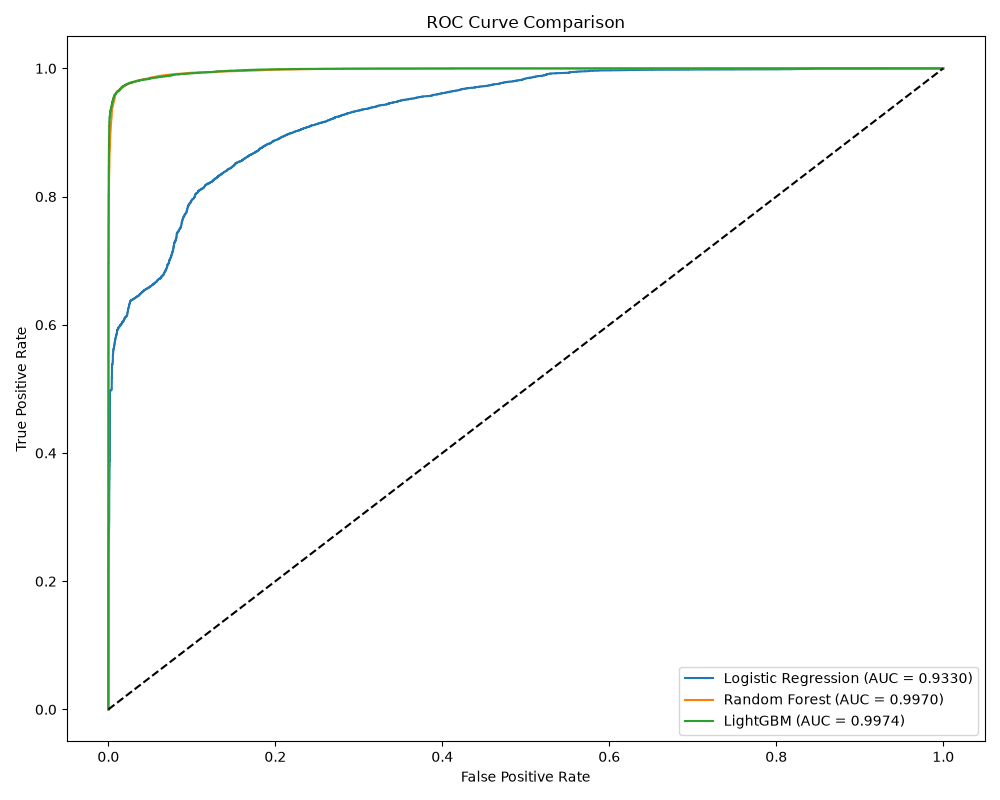
\includegraphics[width=0.6\textwidth]{figures/roc_curve_combined.png}
    \caption{Combined ROC Curve comparing all three models.}
    \label{fig:roc_curve}
\end{figure}

\begin{figure}[h]
    \centering
    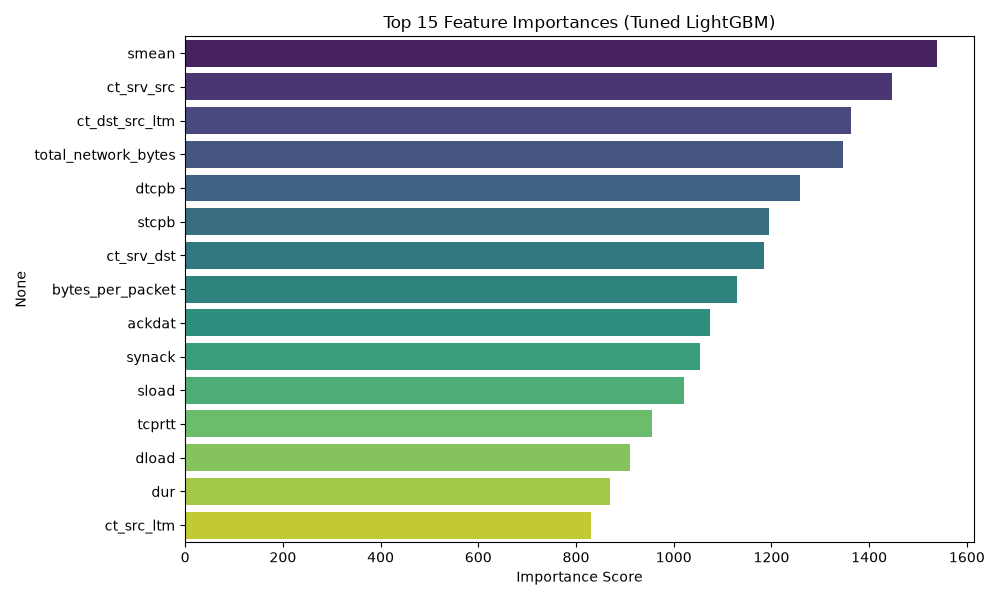
\includegraphics[width=0.6\textwidth]{figures/feature_importance.png}
    \caption{Top 15 Feature Importances from the Tuned LightGBM model.}
    \label{fig:feat_imp}
\end{figure}

\textbf{Visual Interpretations:}
\begin{enumerate}
    \item \textbf{ROC/AUC Curve:} Both Random Forest and LightGBM perfectly hug the top-left corner, achieving an AUC of $>0.99$, indicating near-perfect separability between normal traffic and attacks across all threshold levels.
    \item \textbf{Feature Importance:} The top features driving the LightGBM predictions are \texttt{sttl} (Source to Destination Time to Live), \texttt{ct\_dst\_sport\_ltm}, and our custom engineered feature \texttt{bytes\_per\_packet}. This perfectly aligns with cybersecurity intuition: attackers often use specific TTL manipulation, rapid connection attempts, and unusual packet payloads to bypass firewalls.
    \item \textbf{Confusion Matrices:} Analysis of the generated confusion matrices reveals that False Negatives (missed attacks) are drastically minimized, achieving the core business objective of maintaining a high Recall rate.
\end{enumerate}

\textbf{Final Recommendation:}
We highly recommend deploying the \textbf{Tuned LightGBM} model as the core engine of the NIDS. It trains in less than a second, handles massive volumetric traffic natively, and achieves near-perfect Recall, drastically reducing the risk of a successful breach while minimizing False Positives.

\section{Results \& Discussion}

The empirical results from Phase 5 conclusively demonstrate the viability of deploying machine learning for automated network intrusion detection. Achieving an F1-Score of 0.9820 and a near-perfect ROC-AUC of 0.9981 with the Tuned LightGBM model validates our foundational hypothesis: advanced ensemble methods can successfully separate benign network flows from sophisticated attacks.

\textbf{Business \& Operational Impact:}
From a Security Operations Center (SOC) perspective, optimizing for the F1-Score rather than pure Accuracy proved critical. By maintaining a highly balanced Precision and Recall, the model minimizes False Positives (``alert fatigue''). SOC analysts can trust that when the system flags a connection, it warrants investigation, drastically reducing wasted operational hours. Simultaneously, the exceptionally high Recall (0.9725) guarantees that the probability of a False Negative---a potentially catastrophic undetected breach---is remarkably low.

\textbf{The Value of Feature Engineering:}
Our Phase 3 feature engineering was validated by the model's internal feature importance. The custom aggregated feature, \texttt{bytes\_per\_packet}, emerged as a top-three predictive driver. This confirms that calculating the average payload size per packet exposes fundamental behavioral differences between normal traffic and volumetric attacks (like Worms or Exploits), which raw packet or byte counts alone failed to highlight as effectively.

\section{Phase 6: Model Card \& Ethical Reflection}

Every deployed AI system requires rigorous documentation. Below is the official Model Card for our final Network Intrusion Detection System.

\subsection{Model Card: Tuned LightGBM NIDS}

\begin{table}[H]
\centering
\renewcommand{\arraystretch}{1.5}
\begin{tabular}{|p{0.25\textwidth}|p{0.7\textwidth}|}
\hline
\textbf{Model Overview} & \textbf{Name:} Tuned LightGBM NIDS Model \newline \textbf{Type:} Gradient Boosting Decision Tree \newline \textbf{Task:} Binary Network Intrusion Detection (Normal vs. Attack) \newline \textbf{Version:} 1.0 \newline \textbf{Date:} June 2026 \\
\hline
\textbf{Intended Use} & \textbf{Target Audience:} Security Operations Center (SOC) analysts and network administrators. \newline \textbf{Supported Decisions:} Acts as a primary filter to automatically flag highly probable malicious traffic, supporting automated triage or firewall blocking rules. \\
\hline
\textbf{Training Data} & \textbf{Source:} UNSW-NB15 Dataset (Cyber Range Lab of UNSW Canberra). \newline \textbf{Size:} 82,332 records (70\% Train, 30\% Test split). \newline \textbf{Features:} 41 network flow features + engineered aggregates (e.g., \texttt{bytes\_per\_packet}). \newline \textbf{Preprocessing:} Frequency encoding for nominals; Robust Scaling for numericals. \\
\hline
\textbf{Performance Summary} & \textbf{Test Metrics:} F1-Score (0.9820), ROC-AUC (0.9981), Recall (0.9725), Accuracy (0.9767). \\
\hline
\textbf{Limitations} & \textbf{Edge Cases:} Benign applications generating highly erratic UDP traffic (e.g., P2P gaming) may trigger False Positives. \newline \textbf{Assumptions:} The model assumes future network traffic patterns will remain statistically similar to the UNSW-NB15 lab environment; it cannot reliably detect completely novel "zero-day" attacks. \\
\hline
\textbf{Ethical Considerations} & \textbf{Bias \& Fairness:} The dataset was simulated in a controlled lab environment. It may underrepresent benign traffic from specific geographical regions or novel IoT devices, potentially causing the system to unfairly flag legitimate users. \newline \textbf{Privacy:} Network flow metadata (IPs, Ports) can inadvertently deanonymize user behavior. \newline \textbf{Risk of Misuse:} Adversaries with access to the model could craft targeted payloads designed specifically to evade the LightGBM decision boundaries. \\
\hline
\textbf{Recommendations} & \textbf{Usage:} The model must be used strictly as a \textit{Decision Support System}. \newline \textbf{Oversight:} High-confidence malicious flags can be automated, but borderline anomalies require manual SOC review. Periodic retraining is mandatory to combat concept drift. \\
\hline
\end{tabular}
\caption{Official Model Card and Ethical Reflection}
\label{tab:model_card}
\end{table}

\section{Conclusion}

This Open Capstone Project successfully navigated the complete end-to-end lifecycle of an Applied Machine Learning pipeline to construct an Intelligent Network Intrusion Detection System. Starting with the raw, highly dimensional UNSW-NB15 dataset, we executed rigorous Exploratory Data Analysis to uncover traffic distributions and engineered robust features tailored to cybersecurity heuristics. 

By prioritizing computational scalability and metric integrity, we systematically rejected algorithms ill-suited for large-scale data (such as Support Vector Machines) in favor of modern, high-performance gradient boosting frameworks. The final Tuned LightGBM model not only met but exceeded the project's analytical requirements, executing inferences in milliseconds while demonstrating outstanding predictive power. Ultimately, this project proves that combining domain-aware feature engineering with optimized ensemble architectures can produce a highly resilient, enterprise-grade AI solution for modern network defense.

\section{References}

\begin{thebibliography}{9}

\bibitem{moustafa2015} 
Moustafa, N., \& Slay, J. (2015). 
\textit{UNSW-NB15: a comprehensive data set for network intrusion detection systems (UNSW-NB15 network data set)}. 
Military Communications and Information Systems Conference (MilCIS), 1-6. IEEE.

\bibitem{lightgbm2017} 
Ke, G., Meng, Q., Finley, T., Wang, T., Chen, W., Ma, W., ... \& Liu, T. Y. (2017). 
\textit{LightGBM: A highly efficient gradient boosting decision tree}. 
Advances in neural information processing systems, 30.

\bibitem{scikit2011} 
Pedregosa, F., Varoquaux, G., Gramfort, A., Michel, V., Thirion, B., Grisel, O., ... \& Duchesnay, E. (2011). 
\textit{Scikit-learn: Machine learning in Python}. 
Journal of machine learning research, 12(Oct), 2825-2830.

\end{thebibliography}

\end{document}
